\documentclass [11pt]{article}
\usepackage [T1]{fontenc}
\usepackage[frenchb]{babel}
\usepackage{graphicx}
\usepackage{subcaption}
\AtBeginDocument{\def\labelitemi{$\bullet$}}
\usepackage{amsmath,amsfonts,amssymb}

\renewcommand\thesection{\thepart.\arabic{section}}

\makeatletter
\@addtoreset{section}{part}
\renewcommand{\thesection}{\thepart.\arabic{section}}
\makeatother

\makeatletter
\renewcommand*\l@section{\@dottedtocline{1}{3em}{3.5em}}
\renewcommand*\l@subsection{\@dottedtocline{2}{6.5em}{4em}}
\makeatother

\usepackage{geometry}
\geometry{
a4paper,
total={170mm, 257mm},
left=20mm,
top=20mm,
}
\begin{document}
\begin{titlepage}
   \centering
\vspace{1cm}
\LARGE  Projet E4 : T3D Trachéo sensors \linebreak
\vspace{1.5cm}

\Huge \textbf {Banc de test pour canule de Trachéotomie}

\vspace{4cm}
\centerline{
\includegraphics[scale=0.15]{Logo_ESIEE_Paris.svg.png}}
\vspace{3.5cm}
\Large\textbf{Groupe de Projet :} {Alexandre GUYON Marie AMIOTt, Diane DE BAZELAIRE, Mélanie PRINGENT, Juliette GLERANT}\linebreak

\Large\textbf{Encadrants :} {Mme Gaëlle LISSORGUES et M. Lionel ROUSSEAU}\linebreak

\Large\textbf{Coordinateurs :} {Dr Jean BERGOUNIOUX et M. Antoine PERRIER}\linebreak



\begin{figure}[!h]
\centering
    \begin{subfigure}[h]{0.25\textwidth}
   
\includegraphics[width=\textwidth]{hopital.png} 
    \end{subfigure}
     \begin{subfigure}[h]{0.25\textwidth}
     
\includegraphics[width=\textwidth]{APHP.png} 
    \end{subfigure}
      \begin{subfigure}[h]{0.25\textwidth}
      
\includegraphics[width=\textwidth]{UGE-ESIEE.png} 
    \end{subfigure}
\end{figure}

       

       \vfill
            

            
       \vspace{0.8cm}
     
   
            
     
       \large E4 Biotechnologie et e-santé \linebreak
\normalsize Année universitaire 2020-2021 \linebreak
       \today
            
   
\end{titlepage}


\newpage
\begin{center}
\huge REMERCIEMENTS
\end{center}

\par Avant d'entrer plus en profondeur dans le développement de notre projet de quatrième année, il nous paraît important de commencer notre rapport par des remerciements. \\

En effet, dans un premier temps, nous souhaitons remercier celles et ceux qui nous ont apporté leur aide tout au long de ce projet et sans qui nous n'aurions jamais eu une aussi bonne expérience.\\

Nous tenons a remercier tout particulièrement le Professeur Jean Bourgounioux, médecin meneur et partenaire du projet, pour sa disponibilité, son aide et son écoute au cours de cette étude.\\

Nous adressons également nos vifs remerciements aux professeurs Mme Gaëlle Lissorgues et M. Lionel Rousseau qui nous ont aidé dans la réalisation de notre projet à travers leur suivi régulier, leurs conseils, leur patience et leur empathie durant l'ensemble de ces semaines de travail. \\

Enfin, pour la fourniture des matériels informatiques et médicaux spécifiques, nous remercions l'équipe de l'an dernier, ayant travaillé en première sur ce projet. \\

\newpage
\tableofcontents


\newpage
\section{GLOSSAIRE : Lexique / Variables et Unités }

\begin{itemize}
\item
\textbf{\underline{Aspiration trachéale  :}} Acte de soins consistant à introduire une sonde d'aspiration bronchique dans la lumière d'une canule de trachéotomie, dans le but d'assurer une ventilation adéquate en dégageant les sécrétions muqueuses.

\item 
\textbf{\underline{Canule :}}  Petit tube qu'on introduit dans un orifice naturel ou artificiel pour permettre l'injection de liquides ou le passage d'air. 

\item 
\textbf{\underline{Espace mort anatomique :}} Volume de gaz contenu dans les voies aériennes de la bouche aux bronchioles (alvéoles non incluses)

\item 
\textbf{\underline{Espace mort physiologique :}} Volume de gaz contenu dans les voies aériennes de la bouche aux bronchioles (alvéoles non incluses) qui ne participe pas aux échanges gazeux, chez l'adulte sain il vaut environ 150 ml.

\item 
\textbf{\underline{Glotte :}} Partie du larynx située entre les cordes vocales inférieures.

\item 
\textbf{\underline{Larynx :}}  Organe situé dans le cou, il constitue une partie centrale de l'appareil respiratoire. Conduit qui relie la gorge à la trachée. Le larynx aide à ce que les aliments et les liquides n'entrent pas dans la trachée.

\item 
\textbf{\underline{Matériaux bio-compatibles :}} Matériau toléré par l'organisme.

\item 
\textbf{\underline{Pharynx : }}Cavité où aboutissent les conduits digestifs et respiratoires

\item 
\textbf{\underline{Respiration  :}} Processus biochimique qui permet de libérer l'oxygène de l'air dans les cellules et de produire de l'énergie pour le corps.

\item 
\textbf{\underline{Trachée :}} Portion du conduit respiratoire comprise entre l'extrémité inférieure du larynx et l'origine des bronches.

\item 
\textbf{\underline{Trachéostomie :}} Ablation totale du pharynx  Opération chirurgicale concernant à faire une ouverture dans la trachée afin d'y insérer un tube dans le cas de la présence de voies respiratoires bloquées ou rétrécies. 

\item 
\textbf{\underline{Trachéotomie :}}  Incision chirurgicale de la trachée, destinée à rétablir le passage de l'air et permettant une intubation.

\item 
\textbf{\underline{Ulcération :}} Formation d'un ulcère, c'est-à-dire perte de substance de la peau ou d'une muqueuse sous forme de plaie qui ne cicatrise pas.

\item 
\textbf{\underline{Ventilation :}} Action qui consiste à créer un renouvellement de l'air, par déplacement dans un lieu clos.

\item 
\textbf{\underline{Voies aériennes/respiratoires centrales :}} Elles correspondent aux conduits de gros calibre, à la base de l'arbre bronchique : la trachée présente une surface de 2,5 $cm^{2}$. Suivant les cliniciens, les limites de cette zone s'arrêtent entre la $5^{ème}$ (bronches sous-segmentaires) et la $10^{ème}$ génération de division.

\item 
\textbf{\underline{Voies aériennes/respiratoires inférieures/basses :}} Elles débutent sous le larynx, avec la trachée. Cette dernière se subdivise à son extrémité en deux branches principales, les bronches, qui se jettent dans le poumon gauche et dans le poumon droit.


\item 
\textbf{\underline{Voies aériennes/respiratoires supérieures/hautes :}} Constituées des fosses nasales, du pharynx et du larynx, elles correspondent à la zone de conduction. Elles sont responsables des actions suivantes : humidification, filtration, réglage de la température de l'air inspiré, transport de l'oxygène vers les poumons, olfaction et phonation.

\end{itemize}

\newpage

\section{L'équipe}
\par Afin que l'équipe travaille en harmonie et soit bien organisée, un rôle principal a été distribué à chaque membre du groupe tout au long du projet. Ces rôles ont été répartis en fonction des préférences et connaissances de chacun, ainsi que des tâches à réaliser. 

\newpage
\part{Introduction}
\par 
 La trachéotomie est souvent le dernier recours avant l'admission en unité de réanimation pour les patients atteints de maladies neuromusculaires dont les voies respiratoires supérieures sont atteintes. Le terme "maladie neuromusculaire" regroupe toutes les pathologies affectant le système nerveux périphérique. De plus, la plupart de ces maladies ont une origine génétique. Les sources épidémiologiques sur les pathologies neuromusculaires sont quasi inexistantes en France. Cependant, on estime par exemple les myopathies de Duchenne à 1/3500 naissances, les amyotrophie spinale infantile à  1/6000 - 10 000 naissances et les dystrophies myotoniques de Steinert à  1/10000.\\

D’autre part, la trachéotomie est une des procédures les plus fréquentes en réanimation, et qui est de plus en plus utilisée notamment après la crise du COVID-19. En effet, nombre de malades ont été trachéotomisés pour améliorer leur ventilation et ainsi éviter leur admission dans les services de réanimation. De fait, un patient trachéotomisé requiert beaucoup moins d'assistance par rapport aux patients intubés. Cette intervention aux grands enjeux est donc d’autant plus importante et d’actualité dans le contexte sanitaire récent. \\

Ainsi, dans le cas des jeunes enfants atteints de ces pathologies, la trachéotomie est souvent le moyen pour ces jeunes patients de garder une vie quasi normale. Mais en quoi consiste la trachéotomie ? \\

\begin{figure}[!h]
\centering
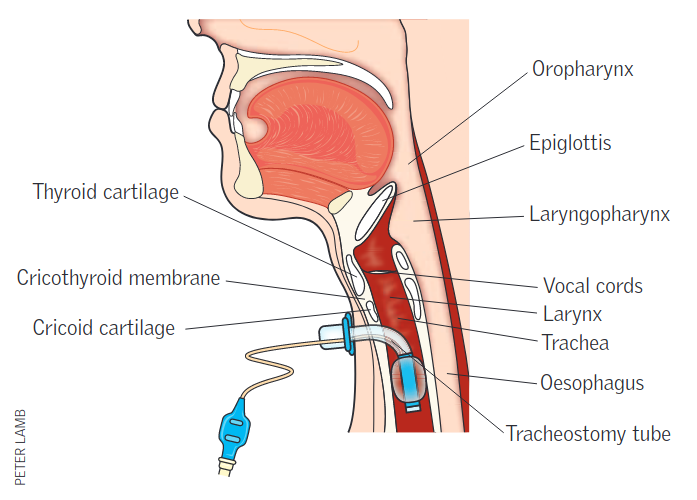
\includegraphics[scale=0.4]{tracheo_principe.png} 
\caption{Positionnement de la canule de trachéotomie}
\label{tracheo}
\end{figure}

\par Ce geste chirurgical consiste à créer une ouverture temporaire de la trachée sous les cordes vocales. On insère ensuite une canule dans cette ouverture, c’est-à-dire un  tube courbé composé de matériaux bio-compatibles. Cette canule permet ainsi au patient de respirer en contournant le nez, la bouche et la gorge. Cette opération peut être réalisée chez les adultes ou les enfants. Néanmoins les canules doivent être adaptées en fonction du patient (variation de la taille de la canule). De plus, les complications divergent quelque peu selon l’âge du patient.  \\

Néanmoins, cette procédure n’est pas sans risques et est source de nombreuses complications. Parmi ces dernières, on retrouve les frottements générés par la présence de la canule au sein de la trachée. La canule, bien que pensée pour s’adapter à la plupart des morphologies, garde une forme standard qui peut générer des frottements et irritations chez les patients en cas de port prolongé. Dans le cas d’un adulte, ce dernier peut aisément vocaliser son inconfort et les soignants peuvent donc réagir en conséquence. Cependant, dans le cas des enfants et d’autant plus chez les très jeunes, ces derniers n’ont pas forcément le réflexe de vocaliser leur inconfort et ont souvent tendance à simplement arracher la canule entraînant leur décès. \\


\newpage
\part{La trachéotomie et ses conséquences}
\section{Qu'est-ce que la trachéotomie ?}

La trachéotomie est une opération chirurgicale très ancienne. Elle consiste à inciser et créer une ouverture temporaire de la trachée, sous le larynx et les cordes vocales, dans laquelle est placée une canule, c'est-à- dire un tube courbé composé de matériaux bio-compatibles. Le but est d'envoyer directement de l'air dans la trachée puis les poumons pour améliorer la ventilation, sans passer par les voies respiratoires hautes. Elle peut être réalisée avec ou sans machine de ventilation.

Cette intervention assez répandue peut être mise en place pour tous types de personnes, enfants comme adultes. Elle est effectuée pour un certain nombre de différents problèmes de respiration et notamment en réanimation. 

Elle est généralement temporaire et nécessaire dans plusieurs situations, en particulier lorsque les voies respiratoires supérieures sont bloquées.

En effet, elle permet une ventilation mécanique prolongée (= elle permet de prendre en charge des patients atteints de maladies neuromusculaires et donc de dépendance ventilatoire) , mais aussi un maintien de l'ouverture de la trachée en cas d'asphyxie, c'est-à-dire en cas d'obstruction des voies respiratoires supérieures. Enfin elle permet également d'aspirer les poussières présentes dans l'air et non filtrées naturellement en cas de déficit de la toux ou encore de protéger la trachée de patients atteints de troubles de la déglutition, notamment des fausses routes. 


La trachéotomie a plusieurs effets sur la ventilation. Elle entraîne une augmentation des résistances et donc une augmentation du travail en ventilation spontanée avec une majoration de la pression expiratoire de pointe.
Étant donné que les voies aériennes supérieures sont court-circuitées, la trachéotomie diminue aussi l’espace mort anatomique des voies respiratoires d’un volume de 150 ml à 20 ml, ce qui diminue la ventilation minute. 
Enfin, elle est à l’origine d’une altération d’un des temps de la toux, c'est-à-dire une altération de la fermeture de la glotte, ce qui impose au patient des aspirations trachéales.
Par conséquent, après le suivi et l’observation de spécialistes, lorsque le patient peut de nouveau respirer par les voies naturelles supérieures et qu’on ne craint plus de complications, comme des troubles importants de la déglutition, la canule peut être retirée.
Une fois celle-ci retirée, l’orifice du pharynx associé se résorbe et se referme, en laissant une petite cicatrice, en général en quelques jours, en fonction du temps passé avec la canule en place.


\newpage
\part{Cahier des charges : objectifs}
vff
\newpage
\part{Recherches sur la trachéotomie : Anatomie}

\newpage
\part{Recherches en électronique: les capteurs }




\newpage
\begin{thebibliography}{99}
\bibitem{ref1}
Bargués-Ribera M, Gokhale CS. Eco-evolutionary agriculture: Host-pathogen dynamics in crop rotations. PLOS Computational Biology. 2020;16(1):e1007546. doi:10.1371/journal.pcbi.1007546
\bibitem{ref1}
Barker CT, Vaidya NK. Modeling HIV-1 infection in the brain. PLOS Computational Biology. 2020;16(11):e1008305. doi:10.1371/journal.pcbi.1008305
\bibitem{ref1}
Bjørnstad ON, Shea K, Krzywinski M, Altman N. Modeling infectious epidemics. Nature Methods. 2020;17(5):455-456. doi:10.1038/s41592-020-0822-z
\bibitem{ref1}
Bjørnstad ON, Shea K, Krzywinski M, Altman N. The SEIRS model for infectious disease dynamics. Nature Methods. 2020;17(6):557-558. doi:10.1038/s41592-020-0856-2
\bibitem{ref1}
Bozic I, Gerold JM, Nowak MA. Quantifying Clonal and Subclonal Passenger Mutations in Cancer Evolution. PLOS Computational Biology. 2016;12(2):e1004731. doi:10.1371/journal.pcbi.1004731
\bibitem{ref1}
Bradford J, Perrin D. A benchmark of computational CRISPR-Cas9 guide design methods. PLOS Computational Biology. 2019;15(8):e1007274. doi:10.1371/journal.pcbi.1007274
\bibitem{ref1}
Caufield JH, Abreu M, Wimble C, Uetz P. Protein Complexes in Bacteria. PLOS Computational Biology. 2015;11(2):e1004107. doi:10.1371/journal.pcbi.1004107
\bibitem{ref1}
Duan G, Walther D. The Roles of Post-translational Modifications in the Context of Protein Interaction Networks. PLOS Computational Biology. 2015;11(2):e1004049. doi:10.1371/journal.pcbi.1004049
\bibitem{ref1}
Fukuyama J, Rumker L, Sankaran K, et al. Multidomain analyses of a longitudinal human microbiome intestinal cleanout perturbation experiment. PLOS Computational Biology. 2017;13(8):e1005706. doi:10.1371/journal.pcbi.1005706
\bibitem{ref1}
Goodsell DS, Jewett A, Olson AJ, Forli S. Integrative modeling of the HIV-1 ribonucleoprotein complex. PLOS Computational Biology. 2019;15(6):e1007150. doi:10.1371/journal.pcbi.1007150
\bibitem{ref1}
Igaev M, Grubmüller H. Microtubule instability driven by longitudinal and lateral strain propagation. PLOS Computational Biology. 2020;16(9):e1008132. doi:10.1371/journal.pcbi.1008132
\bibitem{ref1}
Kønig SM, Rissler V, Terkelsen T, Lambrughi M, Papaleo E. Alterations of the interactome of Bcl-2 proteins in breast cancer at the transcriptional, mutational and structural level. PLOS Computational Biology. 2019;15(12):e1007485. doi:10.1371/journal.pcbi.1007485
\bibitem{ref1}
Koyama S, Horie T, Shinomoto S. Estimating the time-varying reproduction number of COVID-19 with a state-space method. PLOS Computational Biology. 2021;17(1):e1008679. doi:10.1371/journal.pcbi.1008679
\bibitem{ref1}
Lee BY, Bartsch SM, Ferguson MC, et al. The value of decreasing the duration of the infectious period of severe acute respiratory syndrome coronavirus 2 (SARS-CoV-2) infection. PLOS Computational Biology. 2021;17(1):e1008470. doi:10.1371/journal.pcbi.1008470
\bibitem{ref1}
Magzoub MM, Prunello M, Brennan K, Gevaert O. The impact of DNA methylation on the cancer proteome. PLOS Computational Biology. 2019;15(7):e1007245. doi:10.1371/journal.pcbi.1007245
\bibitem{ref1}
Moran R, Keramati M, Dolan RJ. Model based planners reflect on their model-free propensities. PLOS Computational Biology. 2021;17(1):e1008552. doi:10.1371/journal.pcbi.1008552
\bibitem{ref1}
Padmanaban V, Tsehay Y, Cheung KJ, Ewald AJ, Bader JS. Between-tumor and within-tumor heterogeneity in invasive potential. PLOS Computational Biology. 2020;16(1):e1007464. doi:10.1371/journal.pcbi.1007464
\bibitem{ref1}
Qi Y, Zhang B. Predicting three-dimensional genome organization with chromatin states. PLOS Computational Biology. 2019;15(6):e1007024. doi:10.1371/journal.pcbi.1007024
\bibitem{ref1}
Roper M, Fernando C, Chittka L. Insect Bio-inspired Neural Network Provides New Evidence on How Simple Feature Detectors Can Enable Complex Visual Generalization and Stimulus Location Invariance in the Miniature Brain of Honeybees. PLOS Computational Biology. 2017;13(2):e1005333. doi:10.1371/journal.pcbi.1005333
\bibitem{ref1}
Scelsi MA, Napolioni V, Greicius MD, Altmann A, Project (ADSP)  for the ADNI (ADNI) and the ADS. Network propagation of rare variants in Alzheimer’s disease reveals tissue-specific hub genes and communities. PLOS Computational Biology. 2021;17(1):e1008517. doi:10.1371/journal.pcbi.1008517
\bibitem{ref1}
Schmid F, Barrett MJP, Obrist D, Weber B, Jenny P. Red blood cells stabilize flow in brain microvascular networks. PLOS Computational Biology. 2019;15(8):e1007231. doi:10.1371/journal.pcbi.1007231
\bibitem{ref1}
Seoane B, Carbone A. The complexity of protein interactions unravelled from structural disorder. PLOS Computational Biology. 2021;17(1):e1008546. doi:10.1371/journal.pcbi.1008546
\bibitem{ref1}
Shatoff E, Bundschuh R. Single nucleotide polymorphisms affect RNA-protein interactions at a distance through modulation of RNA secondary structures. PLOS Computational Biology. 2020;16(5):e1007852. doi:10.1371/journal.pcbi.1007852
\bibitem{ref1}
Valiente-Mullor C, Beamud B, Ansari I, et al. One is not enough: On the effects of reference genome for the mapping and subsequent analyses of short-reads. PLOS Computational Biology. 2021;17(1):e1008678. doi:10.1371/journal.pcbi.1008678
\bibitem{ref1}
Viswanathan R, Fajardo E, Steinberg G, Haller M, Fiser A. Protein—protein binding supersites. PLOS Computational Biology. 2019;15(1):e1006704. doi:10.1371/journal.pcbi.1006704
\bibitem{ref1}
Wang S, Hottz P, Schechter M, Rong L. Modeling the Slow CD4+ T Cell Decline in HIV-Infected Individuals. PLOS Computational Biology. 2015;11(12):e1004665. doi:10.1371/journal.pcbi.1004665
\bibitem{ref1}
Wu X, Mel GC, Strouse DJ, Mel BW. How Dendrites Affect Online Recognition Memory. PLOS Computational Biology. 2019;15(5):e1006892. doi:10.1371/journal.pcbi.1006892
\bibitem{ref1}
Zhao Z, Sokhansanj BA, Malhotra C, Zheng K, Rosen GL. Genetic grouping of SARS-CoV-2 coronavirus sequences using informative subtype markers for pandemic spread visualization. PLOS Computational Biology. 2020;16(9):e1008269. doi:10.1371/journal.pcbi.1008269
\bibitem{ref1}
Lee C-H, MacKinnon R. Activation mechanism of a human SK-calmodulin channel complex elucidated by cryo-EM structures. Science. 2018;360(6388):508-513. doi:10.1126/science.aas9466
\bibitem{ref1}
Mistry J, Chuguransky S, Williams L, et al. Pfam: The protein families database in 2021. Nucleic Acids Res. 2020;49(D1):D412-D419. doi:10.1093/nar/gkaa913
\bibitem{ref1}
 Becker AD, Wesolowski A, Bjørnstad ON, Grenfell BT. Long-term dynamics of measles in London: Titrating the impact of wars, the 1918 pandemic, and vaccination. PLOS Computational Biology. 2019;15(9):e1007305. doi:10.1371/journal.pcbi.1007305
 \bibitem{ref 1}
Bharti N, Djibo A, Ferrari MJ, et al. MEASLES HOTSPOTS EPIDEMIOLOGICAL CONNECTIVITY. Epidemiol Infect. 2010;138(9):1308-1316. doi:10.1017/S0950268809991385
\bibitem{ref 1}
Earn DJD, Rohani P, Bolker BM, Grenfell BT. A Simple Model for Complex Dynamical Transitions in Epidemics. Science. 2000;287(5453):667-670. doi:10.1126/science.287.5453.667
\bibitem{ref 1}
Kuznetsov YuA, Piccardi C. Bifurcation analysis of periodic SEIR and SIR epidemic models. J Math Biol. 1994;32(2):109-121. doi:10.1007/BF00163027
\bibitem{ref 1}
Tanaka G, Aihara K. Effects of seasonal variation patterns on recurrent outbreaks in epidemic models. Journal of Theoretical Biology. 2013;317:87-95. doi:10.1016/j.jtbi.2012.09.038
\bibitem{ref 1}
Kang PW, Westerlund AM, Shi J, et al. Calmodulin acts as a state-dependent switch to control a cardiac potassium channel opening. Sci Adv. 2020;6(50). doi:10.1126/sciadv.abd6798


\end{thebibliography}
\end{document}




